\documentclass[12pt]{article}

% This first part of the file is called the PREAMBLE. It includes
% customizations and command definitions. The preamble is everything
% between \documentclass and \begin{document}.

\usepackage[margin=1in]{geometry}  % set the margins to 1in on all sides
\usepackage{graphicx}              % to include figures
\usepackage{amsmath}               % great math stuff
\usepackage{amsfonts}              % for blackboard bold, etc
\usepackage{amsthm}                % better theorem environments
\usepackage[rightcaption]{sidecap}
\usepackage{float}

\DeclareMathOperator{\id}{id}


\begin{document}


\nocite{*}


\title{Smoke Detection via Linear Separation}

\author{Banafsheh Rekabdar, Duncan Wilson \\ 
Department of Mathematics and Statistics \\
University of Nevada, Reno}

\maketitle

\begin{abstract}
  This is an implementation of two of the methods presented in Tian, Li et al's paper Smoke Detection in Video: An Image Separation Approach\cite{pap1} on a data set of images from the Lake Tahoe and southern California region. Here we present a matting technique to determine salient regions in large images with small pixel regions corresponding to smoke. This allows for a significant amount the unimportant regions to be filtered out when passing along images to the classifier. We hope for this work to have positive utility in furthering the preprocessing stage of the algorithmic smoke detection pipeline.
\end{abstract}

\newpage
\section{Introduction}

In Tian, Li et al, they propose three novel methods to detect regions of smoke in an image. This directly aids in the preprocessing phase of algorithmic smoke detection and we have implemented two of these solutions on data sets from the Lake Tahoe and the southern California region. Here we will disclose the structure for both of these algorithms that were implemented, followed by some analysis of our results and possibles uses of this work. 

\section{Structuring the Problem}
\label{sect:basics}

\subsection{Background}

The problem of building a system for smoke detection has many sub-problems outlined the smoke detection pipeline. This work is focused on the matting problem, which entails splitting an image into regions (possibly  overlapping) and giving a prediction of whether or not the region contains smoke.

Since wildfires spread quickly this means that there is a great need for them to be detected as quickly as possible. Due to the structure of the classification pipeline, this means the matting phase needs to perform well in the cases where smoke is first appearing and spreading quickly. We've incorporated a correlation model into our algorithms to account for the rapid change which appears in the regions of quickly spreading smoke.      

\subsection{Smoke Structure}

Since the problem of matting simplifies to detecting whether or not a region of pixels is smoke or not, the first thing we must examine is the structure of smoke. In Narasimhan and Nayar (2002)\cite{NN} they lay out multiple atmospheric scattering models of which two are assumed for this work.  

The first of these models is that of attenuation. In physics attenuation refers to the phenomena of a loss of flux when a field passes through a medium. In this context the change in the flux of light through the medium of smoke is of the greatest importance. While  Narasimhan and Nayar explicate a exponential law model, for this application the assumption of attenuation is all that matters. 

The second model which is assumed is that of airlight, which is a phenomena by which light provokes the atmosphere to act like a light source. This is caused by particles in the atmosphere scattering the illumination of the light source. As with the attenuation model, there are analytical solutions relating to the scattering coefficient presented in Narasimhan and Nayar, but again for matting the assumption that smoke will create airlight is what is most important. 

\subsection{Linear Modeling}
Given the two models above, we now will examine the problem's formulation and possible solutions: 
We treat each image as a collection of subsections of pixels $\boldsymbol{f_{t}} \in \mathbb{R}^{N} $. If, as is reasonable, we assume that the scattering coefficient only varies slightly within regions of smoke we can treat regions of the image (represented by $\boldsymbol{f_{t}}$) as a linear combination of the background vector of the image without smoke in it ($\boldsymbol{b_{t}}$) and a smoke vector ($\boldsymbol{s_{t}}$):
\begin{equation}
\boldsymbol{f_{t}} = \alpha_{t}\boldsymbol{s_{t}} + (1-\alpha)\boldsymbol{b_{t}} + {n_{t}}  
\end{equation}
With ${n_{t}} \in \mathbb{R}^{N} $ representing the noise in the model. With the assumption of the airlight model $\boldsymbol{s_{t}}$ can be thought of as the scattering component with an infinite thickness. This seemingly strange assumption allows for the airlight model to be incorporated to be used in this linear fashion. 

In (1), $\alpha_{t}$ can be thought of as a blending parameter that is $\in \left [0,1\right ]$. (1) depends on both the thickness of the smoke as well as the scattering (smoke) coefficient at time $t$. So while the the blending will vary region from region, we will further assume that $\alpha$ won't vary with in a specific region of smoke, due to the likely uniform thickness in a specific small region.  

As the team in the seismology lab have informed us, $\boldsymbol{f_{t}}$ is obtained from a camera which is not moving and due to there being a plethora of non-smoke containing images from the camera we need not doing any background modeling in order to find $\boldsymbol{b_{t}}$.  

This results in the salient region selection can formulated as a two variable estimation problem of $\alpha_{t}$ and $\boldsymbol{s_{t}}$ by minimizing the following: 
\begin{equation}
\min\left \|   \boldsymbol{f_{t}} - \alpha_{t} s_{t} - (1-\alpha_{t} )\boldsymbol{\mathbf{b}_{t}}\right \|^2  s.t. :   \alpha_{t} \in \left [ 0 ,1 \right ]
\end{equation}

But this equation has two unknowns and one equation and thus results in an infinite amount of solutions. So our best hope to estimate both variables is by constraining either $\boldsymbol{b_t}$ or $\boldsymbol{s_{t}}$ and as our background from different cameras will be completely different but in each image the smoke should retain a similar structure, we will constrain $\boldsymbol{s_{t}}$ for the following two methods.   


\section{Local Smoothness}
\label{sect:basics}

\subsection{Model Formulation}
The premise that this model rests on is that a given a small region of smoke there appears to be a great deal of local smoothness. Which in turn means that this region must have roughly similar pixel values. This observation allows us to modify (2) to include a measure of local smoothness: 
\begin{equation}
\min\left \|   \boldsymbol{f_{t}} - \alpha_{t} s_{t} - (1-\alpha_{t} )\boldsymbol{\mathbf{b}_{t}}\right \|^2 +\lambda\sum_{i = 1}^{N} \sum_{j\in\varphi_{i}}(s_{t_i}-s_{t_j})^2 \\ 
\quad
 s.t. :   \alpha_{t} \in \left [ 0 ,1 \right ]
\end{equation}

Now in (3) we see that the minimization also considers the amount of local smoothness present. $\lambda$ can thought of as a tuning parameter by which more or less smoothness of subregions are considered and $\varphi_{i}$ is the local region in which smoothness is assumed and is centered at the $i'th$ pixel.

To make this math more compact and concise we can formulate the second term in the equation with a matrix representation. Let $\boldsymbol{T}$ be an $N$x$M$ matrix with elements $\in \left\{-1,0,1\right\}$. $M$ is decided when picking your size of region $\varphi$. Each the $N$x$i$ element of $\boldsymbol{T}$ equals $1$ and all others $\in \varphi_{i} $ equals $-1$. This means the second term in (3) becomes: 
\begin{equation}
\sum_{i = 1}^{N} \sum_{j\in\varphi_{i}}(s_{t_i}-s_{t_j})^2 = \left \| \boldsymbol{Ts_t} \right \|^2 = \boldsymbol{s^T_tT^TTs_t}=\boldsymbol{s^T_tAs_t} 
\end{equation}
For simplicity's sake we've set $\boldsymbol{A} = \boldsymbol{T^TT}$. Substituting the result of (4) back into (3) we get:
\begin{equation}
\min\left \|   \boldsymbol{f_{t}} - \alpha_{t} s_{t} - (1-\alpha_{t} )\boldsymbol{\mathbf{b}_{t}}\right \|^2 +\lambda\boldsymbol{s^T_sAs} 
\quad
 s.t. :   \alpha_{t} \in \left [ 0 ,1 \right ]
\end{equation}



\subsection{Analytical Solutions}
Due to the under-determined nature of (5) to optimize you must trade off between fixing either ${s_{t}}$ or $\alpha_t$. To solve for ${s_{t}}$, hold $\alpha_t$ constant and set the partial derivative to 0. This results in the following optimal solution to ${s_{t}}$: 
\begin{equation}
\hat{s_t} = (\alpha_t^2\boldsymbol{I} + \lambda\boldsymbol{A_t})^{-1} \alpha_t(\boldsymbol{f_t}-\boldsymbol{b_t} +\alpha_t\boldsymbol{b_t})
\end{equation}
with $\boldsymbol{I}$ being an $N$x$N$ identity matrix. 

We also can derive an optimal solution to $\alpha$ by holding ${s_t}$ constant: 
\begin{equation}
\breve{\alpha }= \frac{(\boldsymbol{b_t-s_t})^T(\boldsymbol{f_t-b_t})}{(\boldsymbol{b_t-s_t})^T(\boldsymbol{s_t-b_t})}
\end{equation}

Due to the constraint that $\alpha \in \left[ 0,1\right]$ in order to obtain the optimal $\alpha$ we constrain $\breve{\alpha }$ by: 
\begin{equation}
\hat{\alpha} =  \begin{cases} 0 & \mbox{if } \breve{\alpha }\mbox{ is} \leq 0 \\ \breve{\alpha }, & \mbox{if }  0<\breve{\alpha }<1\\ 1 & \mbox{if } \breve{\alpha } \mbox{ is} \geq 1 \end{cases}
\end{equation}

So to optimize, oscillate between these two equations until convergence or an upper bound of maximum iterations is reached.   





\section{PCA Model}
\subsection{Model Formulation}

Although the additional term to the minimization eliminates non-smooth sub-regions, it still could fall victim to detecting other regions which are locally smooth as smoke depending on your $\lambda$ parameter in (5). We'd rather have a system which incorporates the features of smoke more specifically and holistically. That leads us to the principle components: 

A given pixel region of pure smoke, with high probability, lies in a lower dimensional sub-space than the totality of the image in which it is contained. Using principle component analysis (Turk and Pentland 1991 \cite{PCA}) we are able to select the salient dimensions which correspond to the subspace. In order to find this subspace you first compute the covariance matrix corresponding to $N$ pure smoke images, which results in an $N$x$N$ matrix, followed by computing the corresponding eigenvalues and vectors. Once you have the eigenvalues, sort the two sets according to magnitude of eigenvalues and select the first eigenvectors up to the upper bound of dimensionality you desire. This results in the information dense dimensions of smoke to be retained and then can be used in the detection process. 

The subspace can be represented as a matrix $\boldsymbol{E} \in \mathbb{R}^{N\times L}$ where $L$ is the reduced dimensionality (thus a general assumption is that $L < N$). As chosen from the aforementioned process, each column of $\boldsymbol{E}$ is an eigenvector corresponding to pure smoke, an "eigensmoke". Assuming that the dimensionality reduction retained all of the salient dimensions (as we'd hope!) we can write the smoke vector at any time-step as $\boldsymbol{s_t} = \boldsymbol{Ey_t}$, where $\boldsymbol{y_t} \in \mathbb{R}^L$ and can be thought of as operational vector by which $\boldsymbol{s_t}$ is projected onto $\boldsymbol{E}$. This means that we can rewrite (2) to incorporate this new formulation of $\boldsymbol{s_t}$:
\begin{equation}
\min\left \|   \boldsymbol{f_{t}} - \alpha_{t} \boldsymbol{Ey_t} - (1-\alpha_{t} )\boldsymbol{\mathbf{b}_{t}}\right \|^2 
\quad
 s.t. :   \alpha_{t} \in \left [ 0 ,1 \right ]
\end{equation}
When holding $\alpha_t$ or $\boldsymbol{y_t}$ constant, this equation becomes quadratic and allows for clean analytical solutions to both $\alpha_t$ and $\boldsymbol{y_t}$ by which $\boldsymbol{s_t}$ can be found via $\boldsymbol{E}$.

\subsection{Analytical Solutions}
When holding $\alpha$ fixed you can set the partial derivative, with respect to $\boldsymbol{s_t}$, to 0 find the optimal $\hat{s_t}$:  
\begin{equation}
\hat{s_t} = \boldsymbol{E}(\alpha_t\boldsymbol{E^TE})^{-1} (\boldsymbol{f_t}-\boldsymbol{b_t} +\alpha_t\boldsymbol{b_t})
\end{equation}

Likewise with $\alpha$: 
\begin{equation}
\breve{\alpha }= \frac{(\boldsymbol{b_t-s_t})^T(\boldsymbol{f_t-b_t})}{(\boldsymbol{b_t-s_t})^T(\boldsymbol{s_t-b_t})}
\end{equation}

To obtain $\hat{\alpha }$ a three case limiting condition as shown in (8) is needed in order for $\breve{\alpha}$ to be within acceptable bounds.   

\subsection{Correlation}
We also included an estimate of correlation in both of our models using the following equation: 
\begin{equation}
c = \frac{(\boldsymbol{f_t}-\bar{\boldsymbol{f_t}})(\boldsymbol{b_t}-\bar{\boldsymbol{b_t}})}{\sqrt{(\boldsymbol{f_t}-\bar{\boldsymbol{f_t}})^2(\boldsymbol{b_t}-\bar{\boldsymbol{b_t}})^2}}
\end{equation}

The only regions which are examined have low correlation, ($c < 0.001$ for PCA and $c < 0.0001$ for local smoothness). This allows us to skip selection for a large amount of regions that stay highly similar in the time from when the background photo was taken to the time which smoke is needed to be detected. Environmental conditions like wind can cause many non-important regions to still possibly be selected even with correlation. 

\section{Results}
Our results vary by camera position and by method used. Overall this matting step in the pipeline, due to the massive size of Tahoe images, is at least minimally helpful by decreasing the number of regions to pass on to the classifier. We've included results from different data sets from both the Tahoe and southern California region. 

In all results that follow the color of the points corresponds with different $\alpha$ values. Specifically green is plotted if $\alpha \geq 0.9$, blue if $0.5 \leq \alpha < 0.9$, and red if $0.3 < \alpha < 0.5$. Also for all results involving the local smoothness model, it should be assumed that $\lambda = 0.7$. (determined as at least semi-optimal via experiment)   

\subsection{Local Smoothness}
The local smoothness model works very well on a majority of the southern California data but, less than perfect on the majority of the images from Tahoe. As the example below shows, the local smoothness model, even when incorporating correlation, still misclassifies many regions in the image as smoke. But it nearly consistently classifies the smoke very well. Due to the rarity of false negatives in the region detection, we feel that this should offer a reliable means to largely reduce the amount of regions needed to be processed by the classifier. 
 

\begin{figure}[H]
\centering
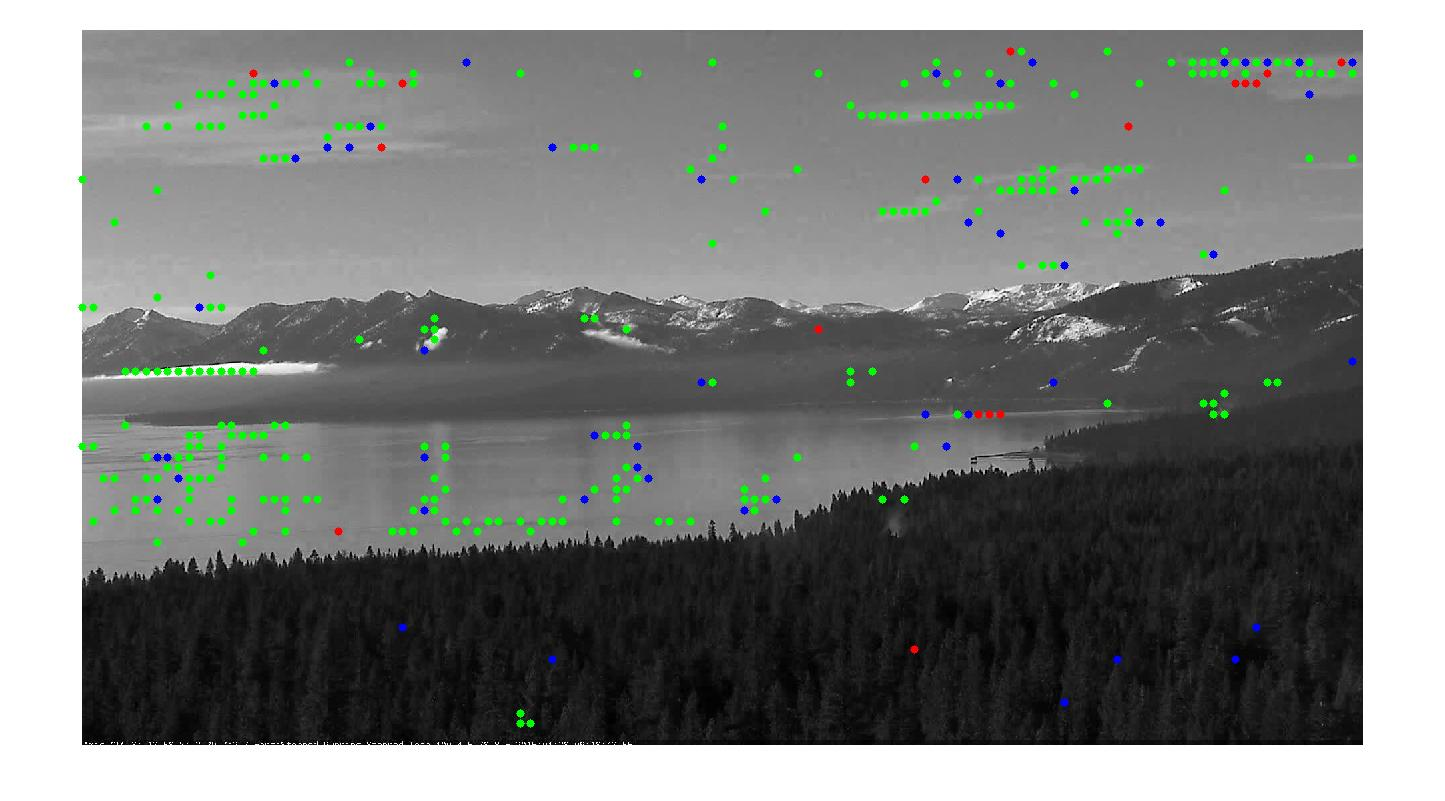
\includegraphics[scale=.2]{LSTahoeHard.jpg}
\caption{This photo from an early stage of a fire from the Tahoe data set}
\end{figure}

\begin{figure}[H]
\centering
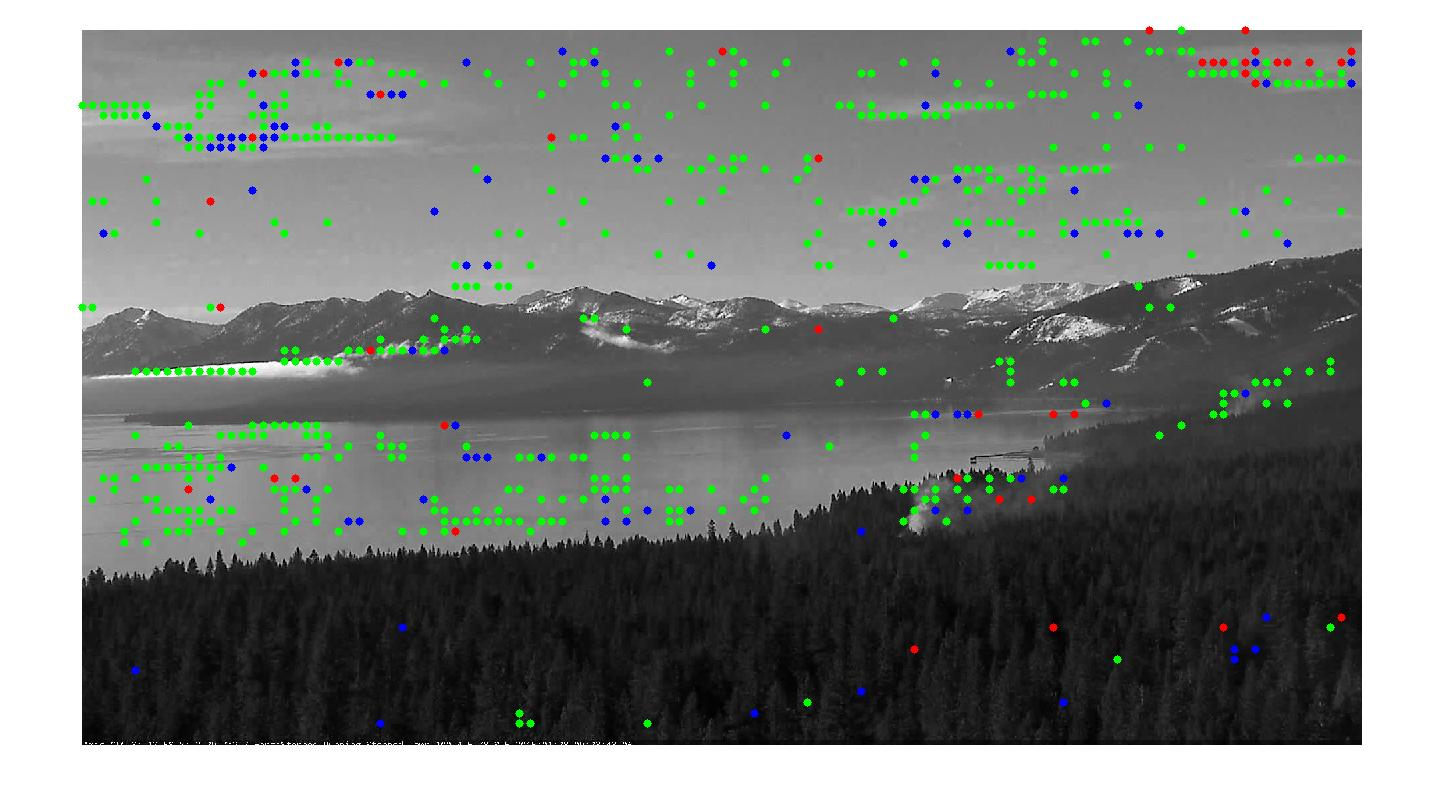
\includegraphics[scale=.2]{LSTahoeEasy.jpg}
\caption{This photo from a later stage of the same fire as above, with regions in both fires on the right of the image well selected for.}

\end{figure}
\begin{figure}[H]
\centering
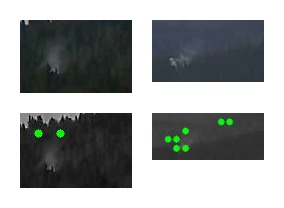
\includegraphics[scale=.5]{lsHardcombined.jpg}
\caption{Close ups of the fire and it's region selection via local smoothness from Figure 1. }
\end{figure}

\begin{figure}[H]
\centering
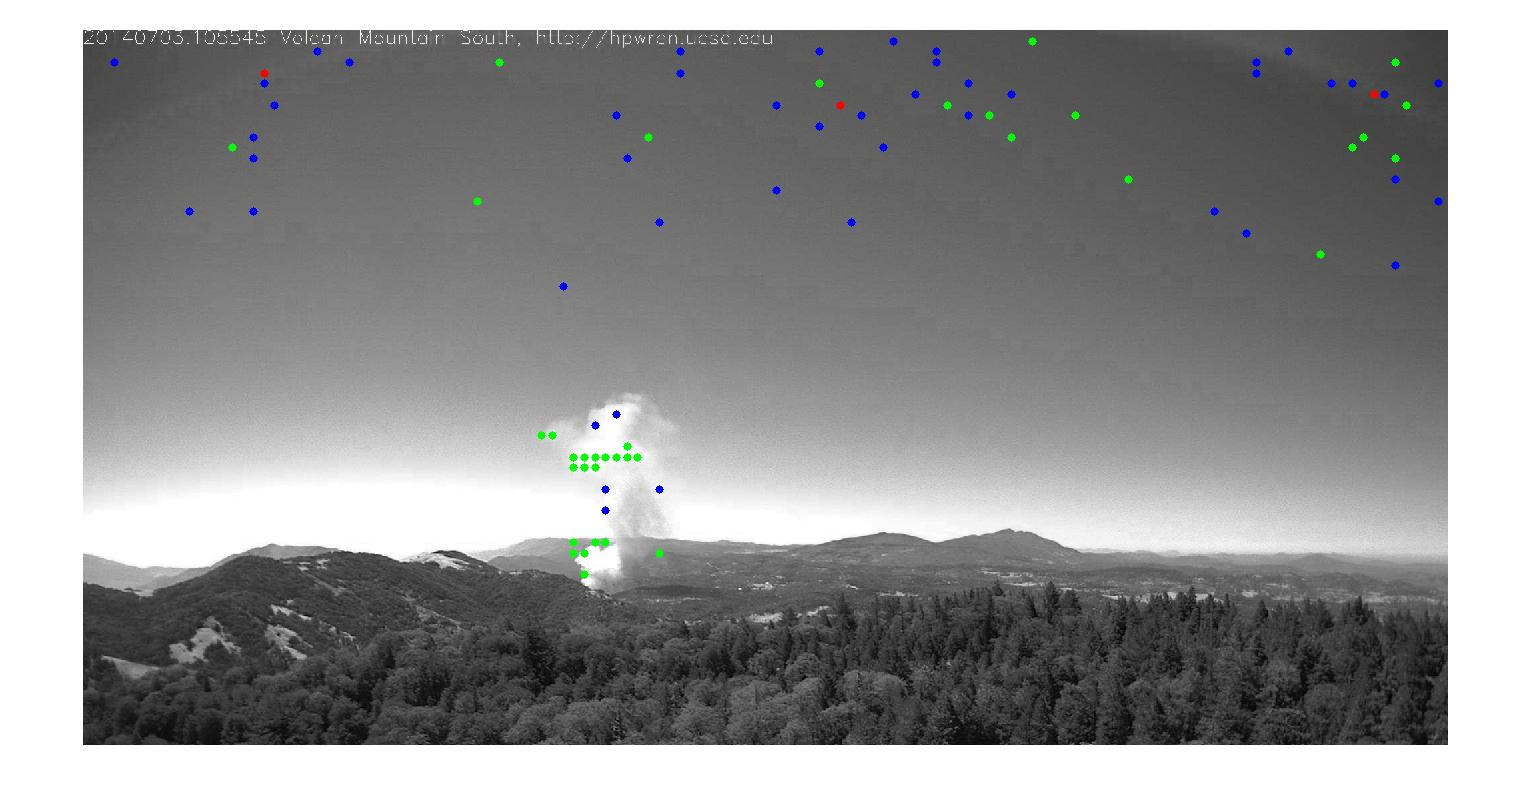
\includegraphics[scale=.2]{smoothGREAT.jpg}
\caption{The best result using local smoothness. (from the southern California data set)}
\end{figure}





\subsection{PCA}

\subsubsection{Eigensmoke}
We collected the training data used in Lian, Ti et al of pure smoke in order to be able to compute the most information rich dimensions.  
\begin{figure}[H]
\centering
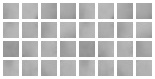
\includegraphics[scale=1]{train.jpg}
\caption{The subset of the pure smoke data set by which the eigensmokes were computed. }
\end{figure}
By computing the covariance matrices and subsequently the eigenvalues and vectors, we were able to compute our "eigensmokes", below are twenty of the eigensmokes.   
\begin{figure}[H]
\centering

\includegraphics[scale=.2]{Z.jpg}
\caption{The top 20 eigensmokes from the training data set}
\end{figure}

\begin{figure}[H]
\centering
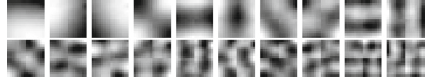
\includegraphics[scale=.8]{papersEigen.png}
\caption{The top 20 eigensmokes from Tian, Li, et al.}

\end{figure}
\subsubsection{PCA results}
Principle component analysis fared quite a bit better in not returning nearly as many false postives as than the local smoothness assumption.  

\begin{figure}[H]
\centering
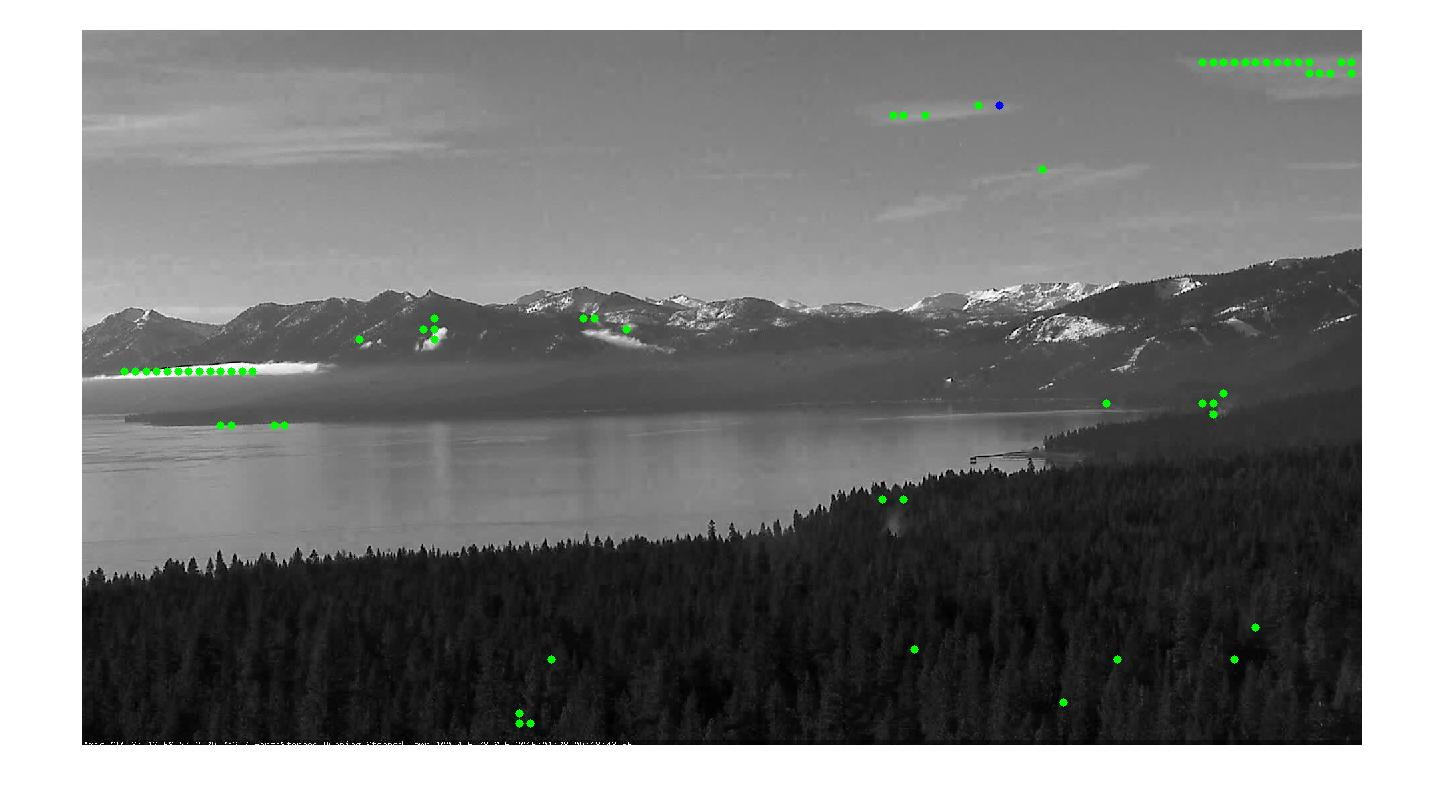
\includegraphics[scale=.2]{pcaTahoeHard.jpg}
\caption{PCA's region selection on the same image as Figure 1. }
\end{figure}

\begin{figure}[H]
\centering
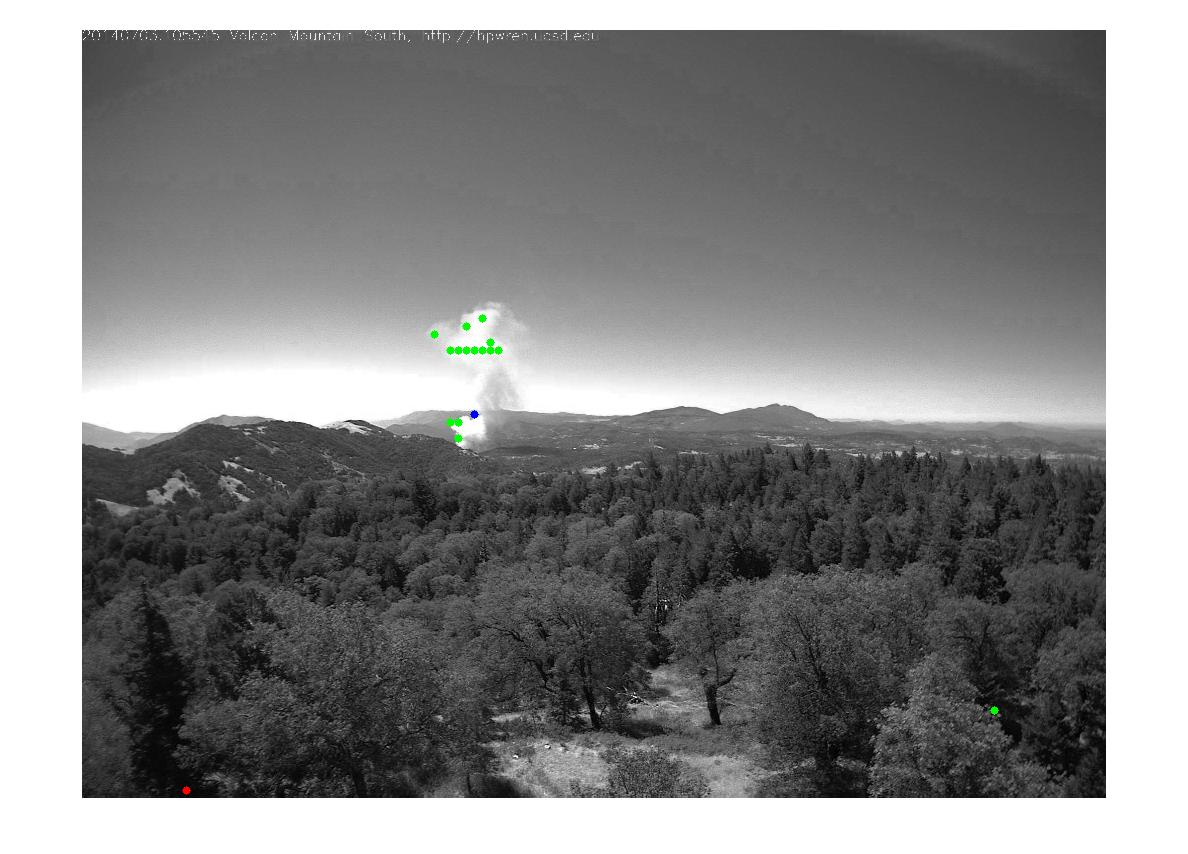
\includegraphics[scale=.2]{pcaGreat.jpg}
\caption{The best result using PCA. (from the southern California data set) }
\end{figure}
There are many more results of both good performance as well as one false positive via PCA on a very cloudy/foggy picture.  

\begin{figure}[H]
\centering
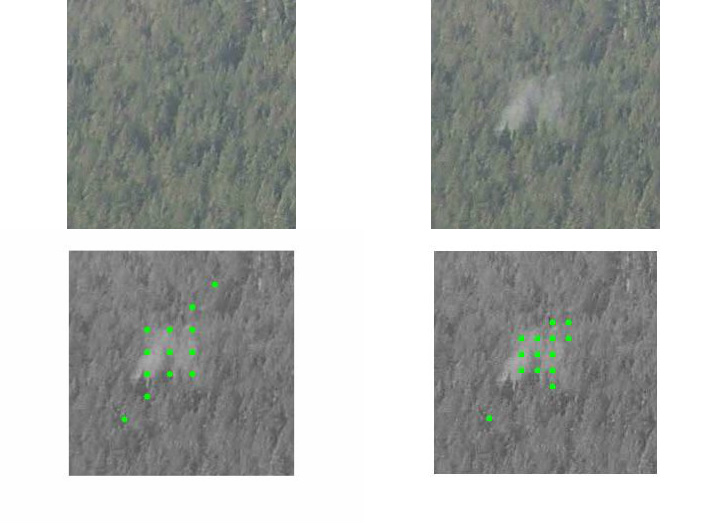
\includegraphics[scale=.2]{combine_images.jpg}
\caption{\newline Top: Background and foreground images Bottom: local smoothness' and PCA's regions}
\end{figure}

\section{Conclusions}
Our results serve as a good matting tool for preprocessing out the salient regions in a given image. Using the principle component analysis method there seems to be a intrinsic flaw in the structure of the eigensmokes. They look a lot like clouds! This means that on clear days there wouldn't be a high rate of cloud containing regions being passed along to the classifier. 

While local smoothness has the drawback of generating lots of false positive, we never found a time that it generated a false negative. Our results imply that PCA is much more accurate but on the other hand, when there is heavy cloud cover or fog can miss the smoke. When combined with the other preprocessing methods, we see this work being reliable enough to be integrated into the final system. 

\section*{Acknowledgements}
We'd like to greatly thank Dr. Raul Rojas for the amazing semester and personal involvement in this work. We're also quite grateful to Tian, Li et al for outlining the methodology used here, as well as sharing their pure smoke data set so that PCA could be used.
\newpage
\bibliographystyle{plain}

\bibliography{references}

\end{document}